\documentclass[12pt]{article}
 
\usepackage[margin=1in]{geometry} 
\usepackage{amsmath,amsthm,amssymb}
\usepackage{hyperref}
\usepackage{graphicx}
\usepackage{xcolor}
\usepackage[many]{tcolorbox}
\tcbuselibrary{listings}
\usepackage{listings}
%jari:
\usepackage{enumitem}

\definecolor{lg}{HTML}{f0f0f0}

\newtcblisting{pycode}{
    colback=lg,
    boxrule=0pt,
    arc=0pt,
    outer arc=0pt,
    top=0pt,
    bottom=0pt,
    colframe=white,
    listing only,
    left=15.5pt,
    enhanced,
    listing options={
        basicstyle=\small\ttfamily,
        keywordstyle=\color{blue},
        language=Python,
        showstringspaces=false,
        tabsize=2,
        numbers=left,
        breaklines=true
    },
    overlay={
        \fill[gray!30]
        ([xshift=-3pt]frame.south west)
        rectangle
        ([xshift=11.5pt]frame.north west);
    }
}

\lstset{
    language=Python,
    basicstyle=\small\ttfamily,
}

 
\begin{document}
 
\title{Exercise 3}
\author{
Jari Mattila - 35260T\\
ELEC-E8125 - Reinforcement Learning}

\maketitle
\section*{Task 1.1}

The training performance plots for Task 1.1 are presented below using a constant value of $\epsilon = 0.2$ in Figure~\ref*{fig:fig1} and reducing the value of $\epsilon$ over time (i.e. using the GLIE formula from the lecture) in Figure~\ref*{fig:fig2}.
\newline

\begin{figure}[h] 
	\centering  % Remember to centre the figure
    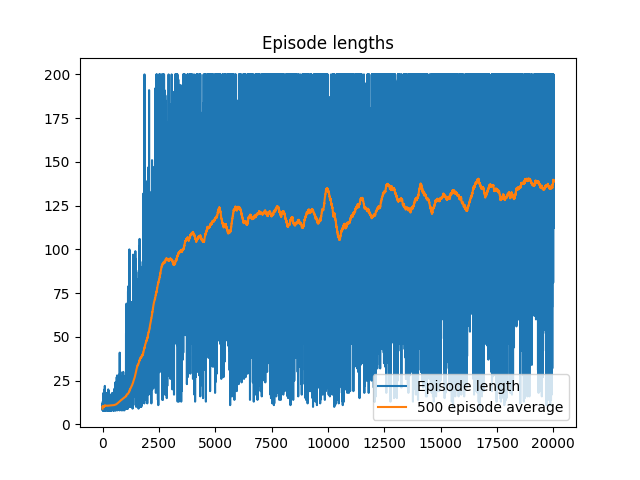
\includegraphics[width=0.9\columnwidth]{img/Figure_1_task1_1_eps-fixed_episode_reward.png}
	\caption{Training performance using a constant value of $\epsilon = 0.2$.}
	\label{fig:fig1}
\end{figure}

\begin{figure}[h] 
	\centering  % Remember to centre the figure
    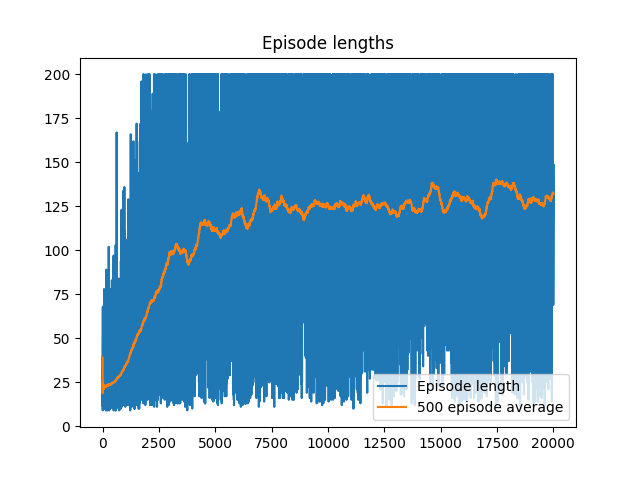
\includegraphics[width=0.9\columnwidth]{img/Figure_1_task1_1_eps-GLIE_episode_reward.png}
	\caption{Training performance using the GLIE formula for $\epsilon$.}
	\label{fig:fig2}
\end{figure}

\pagebreak

\noindent
Source files: qlearning.py, q\_values\_task1\_1.npy, value\_func\_task1\_1.npy

\section*{Task 1.2}

The heatmap from the end of the training is presented in Figure~\ref*{fig:fig3}. From Exercise 1 the states of the cartpole are: \{$x$, $\dot{x}$, $\theta$, $\dot{\theta}$\}. For plotting, the values of the value function are averaged over $\dot{x}$ and $\dot{\theta}$. 
\newline

\begin{figure}[h] 
	\centering  % Remember to centre the figure
    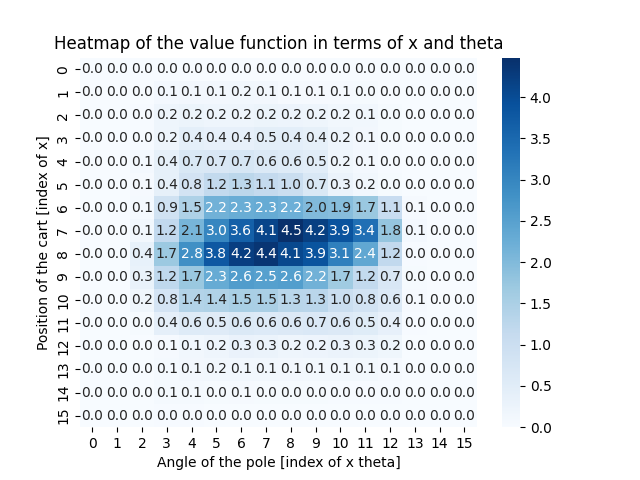
\includegraphics[width=0.9\columnwidth]{img/Figure_2_task1_2_heatmap_blues.png}
	\caption{Heatmap of the value function in terms of $x$ and $\theta$.}
	\label{fig:fig3}
\end{figure}

\section*{Question 1}

What do you think the heatmap would have looked like:

%\begin{itemize}
\begin{enumerate}[label=(\alph*)]
    \item before the training?
   
Before the training Q-values and the value function values are initialized to zero thus the heatmap would show a zero value for each state.

    \item after a single episode?

The positions in the middle row of the heat map would show very small values (around $1..5e^{-3}$) because the initial state indices are as follows: (8, 8, 8, 7) and only the values around the initial state are affected after a single episode.
    
    \item halfway through the training?
    
The values of the value function have not yet converged to the final values, otherwise the heatmap looks very similar to the final heatmap. 

\end{enumerate}
%\end{itemize}


\section*{Task 1.3}

The training performance plots with the greedy policy ($\epsilon=0$) are presented 
in Figure~\ref*{fig:fig4} where the Q function estimates are initialized to 0 and 
Figure~\ref*{fig:fig5} where the initial Q function estimates are set to 50 for all states and actions. 
\newline

\pagebreak


\begin{figure}[h] 
	\centering  % Remember to centre the figure
    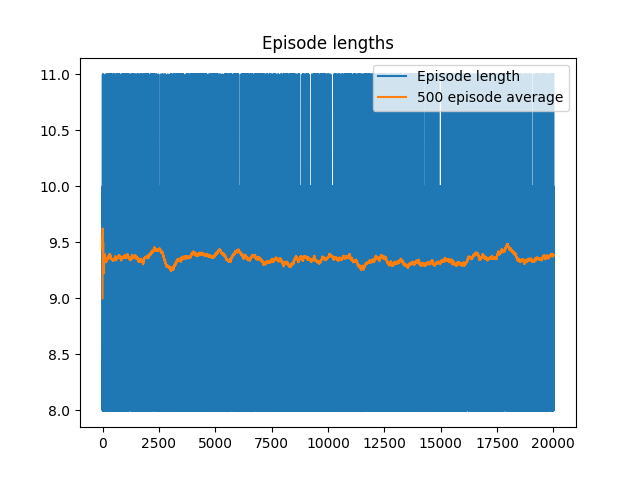
\includegraphics[width=0.9\columnwidth]{img/Figure_4_task1_3a_episode_reward.png}
	\caption{Training performance using $\epsilon$ with zero value (i.e. greedy policy) and 
	keeping the intial estimates of the Q function at 0.}
	\label{fig:fig4}
\end{figure}

\begin{figure}[h] 
	\centering  % Remember to centre the figure
    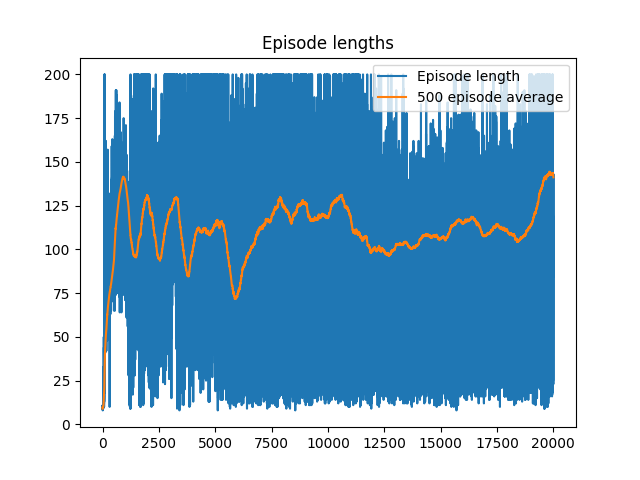
\includegraphics[width=0.9\columnwidth]{img/Figure_5_task1_3b_episode_reward.png}
	\caption{Training performance using $\epsilon$ with zero value (i.e. greedy policy) and 
	setting the initial estimates of the Q function to 50 for all states and actions.}
	\label{fig:fig5}
\end{figure}


\section*{Question 2}

Based on the results you observed in Task 1.3, answer the following questions:

\section*{Question 2.1}

In which case does the model perform better?
\newline

The model performs clearly better in the case of Figure~\ref*{fig:fig5} where 
the initial estimates of the Q function are set to 50 for all states and actions.

\section*{Question 2.2}

Why is this the case, and how does the initialization of Q values affect exploration?
\newline

If the Q values are initialized to zero along with the greedy policy ($\epsilon=0$), the action of zero is always selected according to the optimal policy and the policy has no way of exploring other alternatives. 
Setting the initial Q function estimates to 50 for all states and actions will resolve this bottleneck.

\pagebreak

\section*{Task 2}

The training performance of the lunar lander for Task 2 is presented in Figure~\ref*{fig:fig6}.
\newline

\begin{figure}[h] 
	\centering  % Remember to centre the figure
    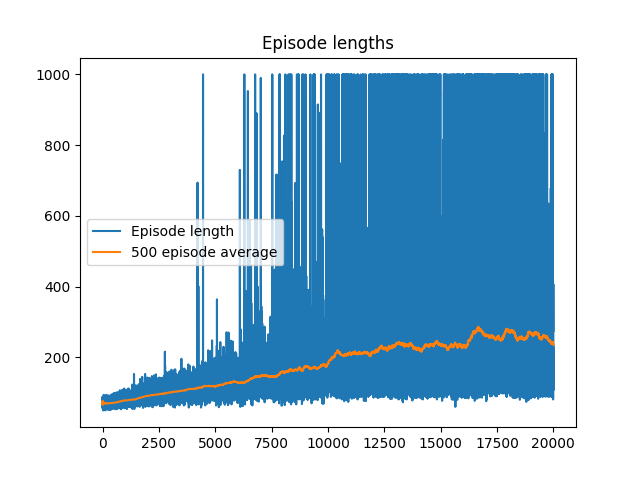
\includegraphics[width=0.9\columnwidth]{img/Figure_7_task2_episode_reward.png}
	\caption{Training performance of the lunar lander using $\epsilon$ with GLIE.}
	\label{fig:fig6}
\end{figure}

%\noindent
%Source files: qlearning.py

\section*{Question 3}

Is the lander able to learn any useful behaviour? Why/why not?
\newline

The lander managed to land successfully a few times so something must have been learned.
The episode lengths of Figure 6 can show that the time without crashing has increased along the number of episodes during training.

\pagebreak



\bibliographystyle{ieeetr}
\bibliography{template}  % Modify template with your bibliography name
\end{document}
